\documentclass[a4paper,11pt]{article}

\newcommand{\authorinfo}{Paul Bienkowski, Konstantin Kobs}
\newcommand{\titleinfo}{Robotics Assignment \#04}

% PREAMBLE ===============================================================

\usepackage[german,ngerman]{babel}
\usepackage[utf8]{inputenc}
\usepackage[T1]{fontenc}
\usepackage[top=1.3in, bottom=1in, left=1.0in, right=0.6in]{geometry}
\usepackage{lmodern}
\usepackage{amssymb}
\usepackage{mathtools}
\usepackage{amsmath}
\usepackage{enumerate}
\usepackage{pgfplots}
\usepackage{breqn}
\usepackage{tikz}
\usepackage{fancyhdr}
\usepackage{multicol}
\usepackage{gensymb}
\allowdisplaybreaks

\usetikzlibrary{calc}
\usetikzlibrary{patterns}

\author{\authorinfo}
\title{\titleinfo}
\date{\today}

\pagestyle{fancy}
\fancyhf{}
\fancyhead[L]{\authorinfo}
\fancyhead[R]{\titleinfo}
\fancyfoot[C]{\thepage}

\begin{document}
\maketitle
\begin {enumerate}
	\item[\textbf{Task 4.1.}]
		% Den gesamten Scheiß habe ich im Skript nicht verstanden, ich habe deshalb auf
		%		https://studywolf.wordpress.com/2013/09/02/robot-control-jacobians-velocity-and-force/
		% ein ganz nettes Tutorial gefunden. :)	
	
		To calculate the Jacobian matrix, we need the position of the end-effector based on the joint angles and the orientation of the end-effector. To get the position, we need to determine the homogeneous transformation from the base to the end-effector point. We can reuse the general transformation matrix given in assignment 2 task 1, because these manipulators are the same. Only $a_i$ needs to be changed to $l_i$. Therefore we have
		
		$${^{0}T_3} = \begin{pmatrix}
			C_{1+2+3} & -S_{1+2+3} & 0 & C_{1+2+3}l_3 + C_{1+2}l_2+C_1l_1\\
			S_{1+2+3} & C_{1+2+3} & 0 & S_{1+2+3}l_3 + S_{1+2}l_2 + S_1l_1\\
			0 & 0 & 1 & 0\\
			0 & 0 & 0 & 1
		\end{pmatrix}$$
		
		From this matrix, we can easily extract the position of the end-effector, which is
		
		$$\begin{pmatrix}
			x \\
			y \\
			z
		\end{pmatrix} = \begin{pmatrix}
			C_{1+2+3}l_3 + C_{1+2}l_2+C_1l_1\\
			S_{1+2+3}l_3 + S_{1+2}l_2 + S_1l_1\\
			0
		\end{pmatrix}$$
		
		The orientation of the end-effector is easy to determine. Because the manipulator just moves in the $(x,y)$-plane, we can set the orientation vector to
		
		$$\begin{pmatrix}
			\omega_x \\
			\omega_y \\
			\omega_z
		\end{pmatrix} = \begin{pmatrix}
			0 \\
			0 \\
			\theta_1 + \theta_2 + \theta_3
		\end{pmatrix}$$
		
		with $\omega$ denotes the angular velocity. Now we can calculate the Jacobian matrices $J_v$ and $J_w$ and from this the resulting Jacobian matrix $J$, which are all partial derivatives of both determined vectors:
		
		\begin{align*}
			J_v &= \begin{pmatrix}
				\frac{\partial x}{\partial \theta_1} & \frac{\partial x}{\partial \theta_2} & \frac{\partial x}{\partial \theta_3} \\
				\frac{\partial y}{\partial \theta_1} & \frac{\partial y}{\partial \theta_2} & \frac{\partial y}{\partial \theta_3} \\
				\frac{\partial z}{\partial \theta_1} & \frac{\partial z}{\partial \theta_2} & \frac{\partial z}{\partial \theta_3}
			\end{pmatrix} \\
			&= \begin{pmatrix}
				-S_{1+2+3}l_3 - S_{1+2}l_2 - S_1l_1 & -S_{1+2+3}l_3 - S_{1+2}l_2 & -S_{1+2+3}l_3\\
				C_{1+2+3}l_3 + C_{1+2}l_2 + C_1l_1 & C_{1+2+3}l_3 + C_{1+2}l_2 & C_{1+2+3}l_3\\
				0 & 0 & 0
			\end{pmatrix}\\
			J_w &= \begin{pmatrix}
				\frac{\partial \omega_x}{\partial \theta_1} & \frac{\partial \omega_x}{\partial \theta_2} & \frac{\partial \omega_x}{\partial \theta_3} \\
				\frac{\partial \omega_y}{\partial \theta_1} & \frac{\partial \omega_y}{\partial \theta_2} & \frac{\partial \omega_y}{\partial \theta_3} \\
				\frac{\partial \omega_z}{\partial \theta_1} & \frac{\partial \omega_z}{\partial \theta_2} & \frac{\partial \omega_z}{\partial \theta_3}
			\end{pmatrix} \\
			&= \begin{pmatrix}
				0 & 0 & 0 \\
				0 & 0 & 0 \\
				1 & 1 & 1 \\
			\end{pmatrix}\\
			J &= \begin{pmatrix}
				J_v\\
				J_w
			\end{pmatrix}\\
			&= \begin{pmatrix}
				-S_{1+2+3}l_3 - S_{1+2}l_2 - S_1l_1 & -S_{1+2+3}l_3 - S_{1+2}l_2 & -S_{1+2+3}l_3\\
				C_{1+2+3}l_3 + C_{1+2}l_2 + C_1l_1 & C_{1+2+3}l_3 + C_{1+2}l_2 & C_{1+2+3}l_3\\
				0 & 0 & 0\\
				0 & 0 & 0 \\
				0 & 0 & 0 \\
				1 & 1 & 1 \\
			\end{pmatrix}\\
		\end{align*}
		
		
	\item[\textbf{Task 4.2.}]
		\begin{enumerate}
			\item[1)] The visualization can be found in the following figure. The grey area that looks like a DVD is the reachable workspace of the arm. The red area depicts the space the second link can reach.
			\begin{center}
				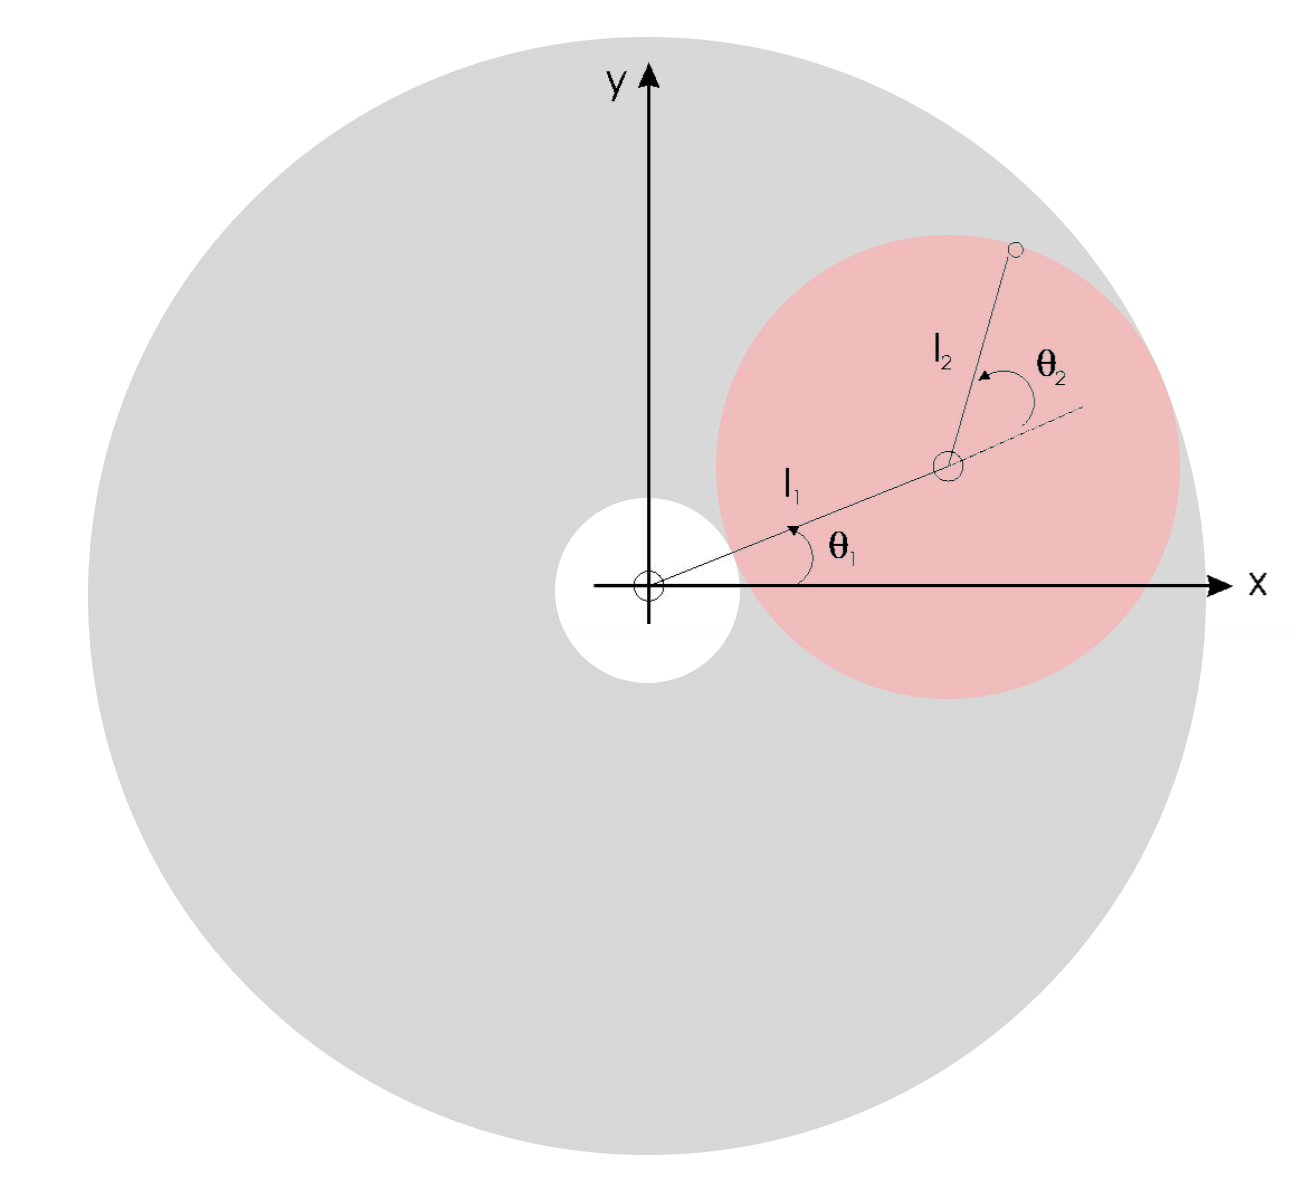
\includegraphics[scale=0.2]{4-2-1.png}
			\end{center}
			
			\item[2)]
				For the calculation of the Jacobian matrix, we need to get (again) the position and orientation of the end effector. The orientation is again as easy to determine as in 4.1:
				$$\begin{pmatrix}
					\omega_x \\
					\omega_y \\
					\omega_z
				\end{pmatrix} = \begin{pmatrix}
					0 \\
					0 \\
					\theta_1 + \theta_2
				\end{pmatrix}$$
				
				The transformation matrix for this manipulator can be determined by calculating:
				
				\begin{align*}
					{^0T_1} &= Rot_{z}(\theta_1) \cdot Trans_{x_1}(l_1)\\
					&= \begin{pmatrix}
						C_1 & -S_1 & 0 & l_1 \cdot C_1\\
						S_1 & C_1 & 0 & l_1 \cdot S_1\\
						0 & 0 & 1 & 0\\
						0 & 0 & 0 & 1
					\end{pmatrix}\\
					{^1T_2} &= Rot_{z}(\theta_2) \cdot Trans_{x_2}(l_2)\\
					&= \begin{pmatrix}
						C_2 & -S_2 & 0 & l_2 \cdot C_2\\
						S_2 & C_2 & 0 & l_2 \cdot S_2\\
						0 & 0 & 1 & 0\\
						0 & 0 & 0 & 1
					\end{pmatrix}\\
					\begin{pmatrix}
						x \\
						y \\
						z \\
						1
					\end{pmatrix} &= {^0T_1} \cdot {^1T_2} \cdot \begin{pmatrix}
						0 \\
						0 \\
						0 \\
						1
					\end{pmatrix}\\
					&= \begin{pmatrix}
						C_1 \cdot C_2 \cdot l_2 - S_1 \cdot S_2 \cdot l_2 + C_1 \cdot l_1\\
						S_1 \cdot C_2 \cdot l_2 + C_1 \cdot S_2 \cdot l_2 + S_1 \cdot l_1\\
						0 \\
						1
					\end{pmatrix}\\
					&\overset{\text{sum formulas}}{=} \begin{pmatrix}
						l_2 \cdot C_{1+2} + C_1 \cdot l_1\\
						l_2 \cdot S_{1+2} + S_1 \cdot l_1\\
						0 \\
						1
					\end{pmatrix}\\
				\end{align*}
				
				Now we construct the two parts of the final Jacobian matrix with the partial derivatives and can then put them together to get the Jacobian matrix.
				
				\begin{align*}
					J_v &= \begin{pmatrix}
						\frac{\partial x}{\partial \theta_1} & \frac{\partial x}{\partial \theta_2} \\
						\frac{\partial y}{\partial \theta_1} & \frac{\partial y}{\partial \theta_2} \\
						\frac{\partial z}{\partial \theta_1} & \frac{\partial z}{\partial \theta_2}
					\end{pmatrix} \\
					&= \begin{pmatrix}
						- l_2 \cdot S_{1+2} - S_1 \cdot l_1 & - l_2 \cdot S_{1+2}\\
						l_2 \cdot C_{1+2} + C_1 \cdot l_1 & l_2 \cdot C_{1+2}\\
						0 & 0
					\end{pmatrix}\\
					J_w &= \begin{pmatrix}
						\frac{\partial \omega_x}{\partial \theta_1} & \frac{\partial \omega_x}{\partial \theta_2} \\
						\frac{\partial \omega_y}{\partial \theta_1} & \frac{\partial \omega_y}{\partial \theta_2} \\
						\frac{\partial \omega_z}{\partial \theta_1} & \frac{\partial \omega_z}{\partial \theta_2}
					\end{pmatrix} \\
					&= \begin{pmatrix}
						0 & 0 \\
						0 & 0 \\
						1 & 1 \\
					\end{pmatrix}\\
					J &= \begin{pmatrix}
						J_v\\
						J_w
					\end{pmatrix}\\
					&= \begin{pmatrix}
						- l_2 \cdot S_{1+2} - S_1 \cdot l_1 & - l_2 \cdot S_{1+2}\\
						l_2 \cdot C_{1+2} + C_1 \cdot l_1 & l_2 \cdot C_{1+2}\\
						0 & 0\\
						0 & 0 \\
						0 & 0 \\
						1 & 1 \\
					\end{pmatrix}\\
				\end{align*}
				
				
			
			\item[3)]
			
			\item[4)]
			
		\end{enumerate}				
		
		
	\item[\textbf{Task 4.3.}]

	\item[\textbf{Task 4.4.}]
	
\end {enumerate}
\end{document}
